\chapter{PHÂN TÍCH BÀI TOÁN THỰC TẾ}

\section{Phát biểu bài toán}

Bài toán nhận dạng biển số xe được xác định là bài toán thị giác máy tính, trong đó hệ thống tiếp nhận ảnh tĩnh, tệp video hoặc luồng camera trực tiếp có chứa phương tiện và tự động trích xuất thông tin biển số. Trọng tâm của đề tài là biển số xe ô tô (biển 1 dòng và biển 2 dòng); biển số xe máy được đưa vào như phần mở rộng do tập dữ liệu sử dụng đã có sẵn nhóm ảnh này.

\noindent\textbf{Về bản chất, bài toán gồm hai nhiệm vụ liên tiếp.}
\nopagebreak

\noindent\textbf{Nhiệm vụ 1: Phát hiện biển số xe trong hình ảnh.}
\nopagebreak

Cho ảnh đầu vào $I$, hệ thống cần xác định ảnh có chứa biển số hay không. Nếu có, hệ thống dự đoán vị trí biển số bằng một hộp chữ nhật bao quanh, kèm theo loại biển (1 dòng hoặc 2 dòng):
\[
  B = (x_{\min},\, y_{\min},\, x_{\max},\, y_{\max},\, \text{conf},\, \text{loại biển})
\]
trong đó $(x_{\min}, y_{\min})$ là góc trên bên trái, $(x_{\max}, y_{\max})$ là góc dưới bên phải và $\text{conf}$ là điểm tin cậy của dự đoán.

\noindent\textbf{Nhiệm vụ 2: Nhận dạng ký tự trên biển số.}
\nopagebreak

Sau khi xác định được vùng biển số, hệ thống cắt vùng ảnh đó và chuyển cho mô hình nhận dạng ký tự. Mô hình trả về chuỗi ký tự cùng độ tin cậy của từng ký tự. Ví dụ, với biển số ``30A-123.45'', kết quả mong muốn là chuỗi chuẩn hóa ``30A12345''; dấu gạch và dấu chấm được thêm lại ở bước hiển thị.

Khi đầu vào là video, hai nhiệm vụ trên được bổ sung bước theo dõi phương tiện qua nhiều khung hình để mỗi xe chỉ sinh ra một bản ghi và kết quả được tổng hợp từ nhiều lần đọc.

\section{Phân tích tập dữ liệu VNLP}

\subsection{Nguồn gốc và cấu trúc}

Nhóm sử dụng tập dữ liệu \textbf{VNLP (Vietnamese License Plate)} do nhóm tác giả Phạm Thế Anh và cộng sự công bố~\cite{pham2023,trinh2022}. Theo mô tả của tác giả, phần lớn ảnh được chụp tại một trung tâm đăng kiểm phương tiện ở Việt Nam. Bộ dữ liệu gồm 37.297 ảnh, chia thành ba thư mục:

\begin{table}[H]
\centering
\small
\begin{tabularx}{\textwidth}{|>{\RaggedRight}p{3.4cm}|>{\centering\arraybackslash}p{1.7cm}|>{\centering\arraybackslash}p{2.0cm}|>{\RaggedRight\arraybackslash}X|}
\hline
\textbf{Thư mục} & \textbf{Số ảnh} & \textbf{Số biển khác nhau} & \textbf{Đặc điểm} \\
\hline
\texttt{one\_row} (ô tô 1 dòng) & 19.086 & 16.521 & Ảnh chụp cận đầu/đuôi xe, biển chiếm phần lớn khung hình \\
\hline
\texttt{two\_rows} (ô tô 2 dòng) & 12.618 & 11.648 & Ảnh toàn thân xe con, xe tải, xe khách; biển nhỏ trong khung hình \\
\hline
\texttt{two\_rows\_label\_} \texttt{xe\_may} (xe máy) & 5.593 & 3.227 & Ảnh từ camera IP đặt thấp phía sau xe máy, nhiều khung hình liên tiếp của cùng một xe \\
\hline
\textbf{Tổng} & \textbf{37.297} & \textbf{20.911} & 10.465 biển có mặt ở cả \texttt{one\_row} và \texttt{two\_rows} \\
\hline
\end{tabularx}
\caption{Cấu trúc tập dữ liệu VNLP (thống kê từ danh sách tệp của bộ dữ liệu)}
\label{tab:vnlp_structure}
\end{table}

Hình~\ref{fig:vnlp_samples} minh họa ảnh đại diện của ba nhóm, trong đó khung đỏ là hộp biển số được vẽ lại từ nhãn gốc.

Tổng số biển khác nhau của cả bộ (20.911) nhỏ hơn nhiều so với tổng của ba thư mục cộng lại. Nguyên nhân là \textbf{10.465 biển xuất hiện ở cả hai thư mục ô tô}: cùng một xe được chụp đầu xe (biển dài, thư mục \texttt{one\_row}) và đuôi xe (biển vuông, thư mục \texttt{two\_rows}). Đặc điểm này ảnh hưởng trực tiếp đến cách chia dữ liệu (Mục~\ref{sec:vnlp_issues}).

\begin{figure}[H]
\centering
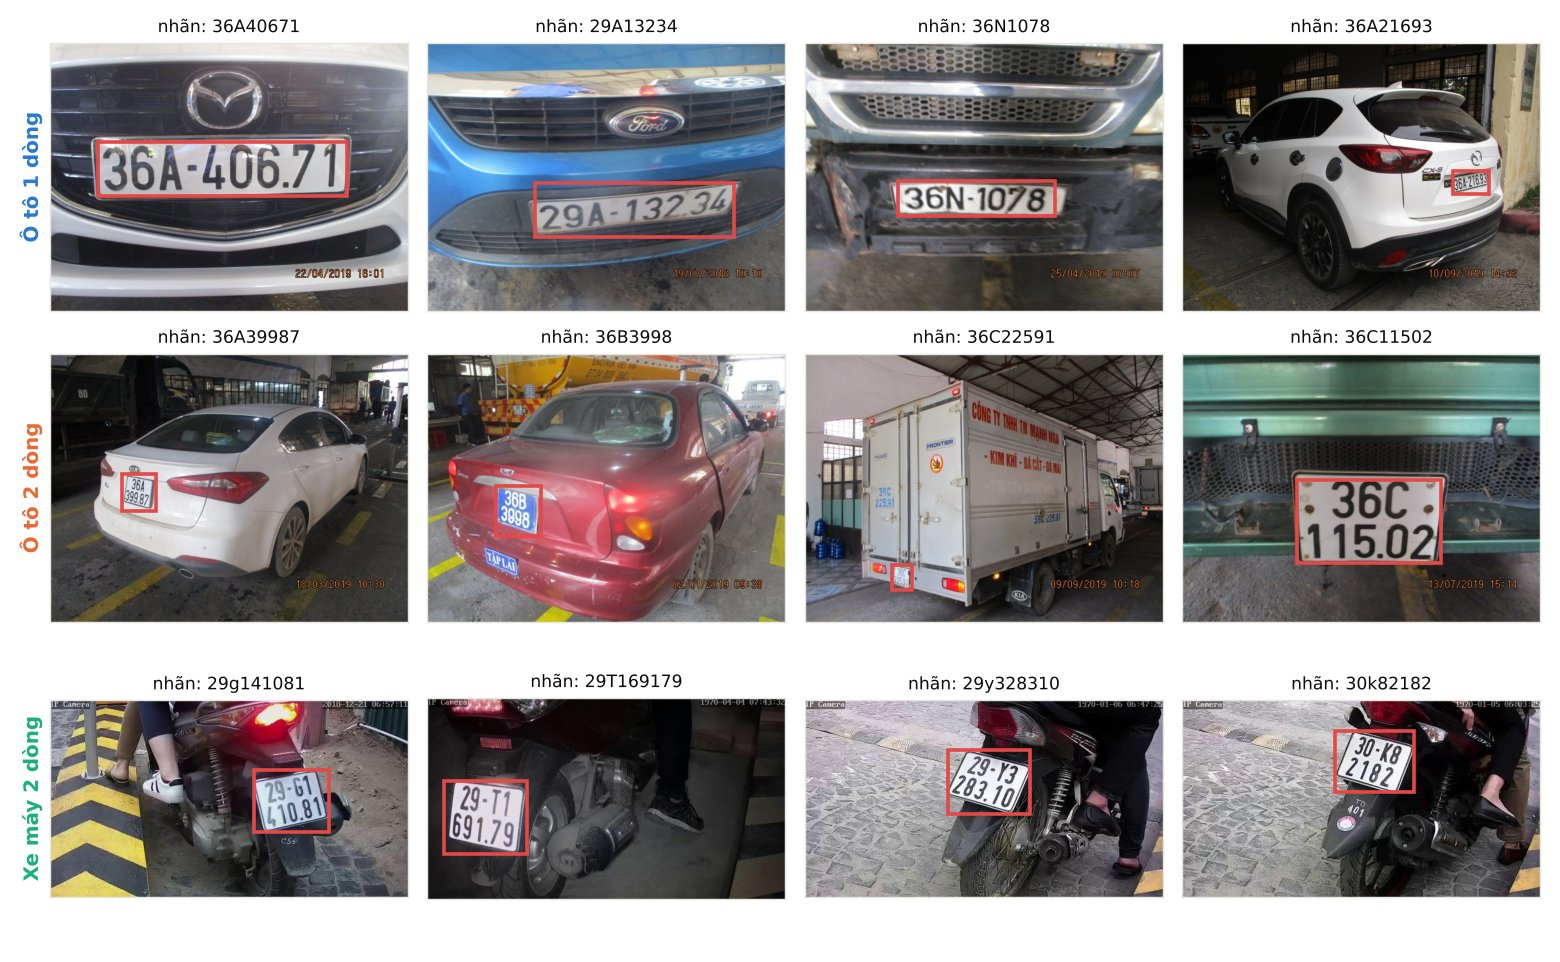
\includegraphics[width=\textwidth]{images/dataset/vnlp_samples.jpg}
\caption{Ảnh mẫu của ba nhóm dữ liệu VNLP (khung đỏ vẽ theo nhãn gốc)}
\label{fig:vnlp_samples}
\end{figure}

\subsection{Định dạng nhãn}

VNLP không có tệp nhãn riêng; toàn bộ thông tin nhãn được mã hóa trong tên tệp ảnh, các trường phân tách bằng dấu gạch dưới. Ví dụ với tệp \texttt{1\_1463\_1\_36C09130\_116\_312\_208\_368.jpg}:

\begin{itemize}
  \item Ba trường đầu (\texttt{1\_1463\_1}) là mã nội bộ, không dùng cho huấn luyện. Trường thứ ba nhận giá trị 1 với biển 1 dòng và 0 với biển 2 dòng.
  \item Trường thứ tư (\texttt{36C09130}) là chuỗi ký tự biển số, đã bỏ dấu gạch và dấu chấm.
  \item Bốn trường cuối (\texttt{116\_312\_208\_368}) là tọa độ hộp biển số.
\end{itemize}

Tài liệu đi kèm bộ dữ liệu ghi bốn số cuối là ``góc trên trái và chiều rộng, chiều cao''. Khi vẽ lại nhãn lên ảnh (Hình~\ref{fig:vnlp_samples}), nhóm xác nhận bốn số này thực chất là \textbf{tọa độ hai góc} $(x_{\min}, y_{\min}, x_{\max}, y_{\max})$: cách hiểu theo chiều rộng, chiều cao làm hộp vượt ra ngoài ảnh rộng 640 điểm ảnh. Đây là chi tiết bắt buộc phải xử lý đúng khi chuyển sang định dạng YOLO.

Trong mẫu 93 ảnh được kiểm tra, mọi ảnh có chiều rộng 640 điểm ảnh, chiều cao 480, 360 hoặc 352 điểm ảnh.

\subsection{Thống kê phân bố}

Hình~\ref{fig:vnlp_stats} tổng hợp các thống kê chính, tính trên toàn bộ 37.297 nhãn.

\begin{figure}[H]
\centering
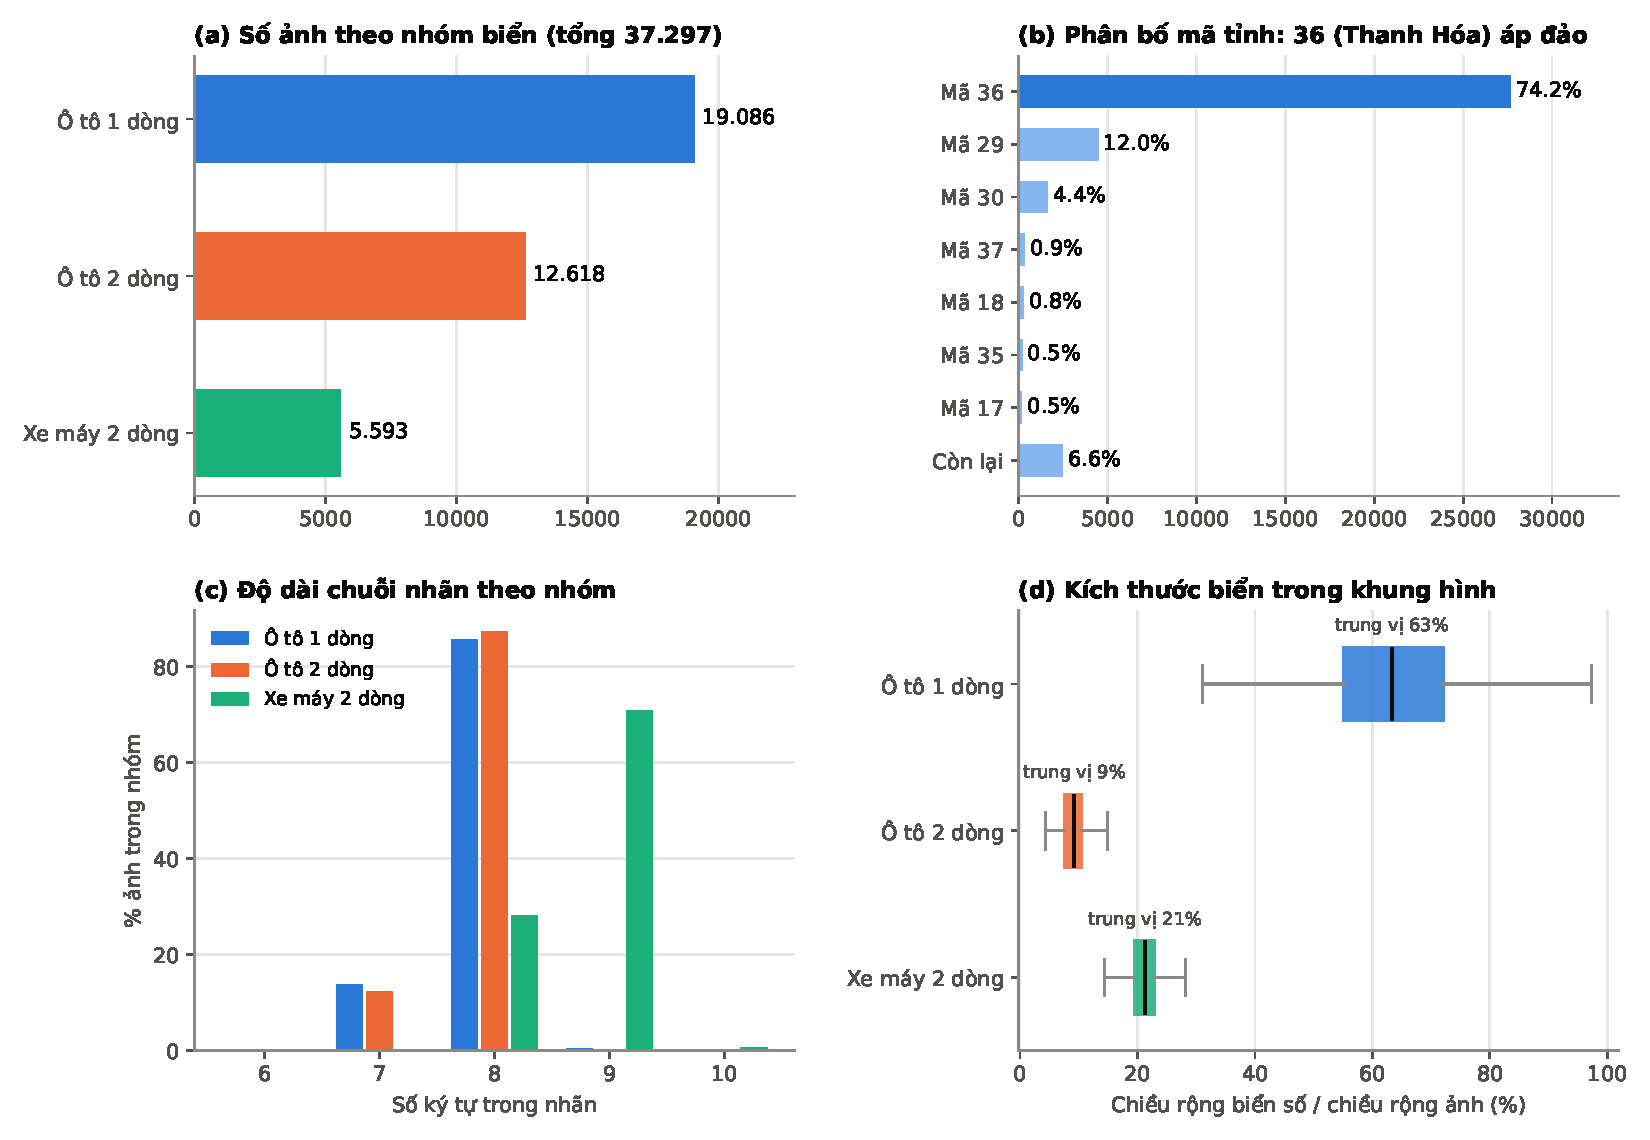
\includegraphics[width=\textwidth]{images/dataset/vnlp_stats.pdf}
\caption{Thống kê tập VNLP: (a) số ảnh theo nhóm, (b) mã tỉnh, (c) độ dài nhãn, (d) kích thước biển so với ảnh}
\label{fig:vnlp_stats}
\end{figure}

Từ Hình~\ref{fig:vnlp_stats} có thể rút ra:

\begin{itemize}
  \item \textbf{Mất cân bằng vùng miền:} biển mã 36 (Thanh Hóa) chiếm 74,2\% toàn bộ dữ liệu và khoảng 87\% ở hai nhóm ô tô; nhóm xe máy chủ yếu là mã 29 (Hà Nội). Các mã tỉnh khác rất ít mẫu.
  \item \textbf{Độ dài chuỗi khác nhau theo nhóm:} biển ô tô chủ yếu dài 8 ký tự (khoảng 86\%) hoặc 7 ký tự (biển cũ 4 số); biển xe máy chủ yếu dài 9 ký tự do seri gồm chữ và số (ví dụ \texttt{29G1-410.81}).
  \item \textbf{Kích thước biển chênh lệch rất lớn:} ở nhóm 1 dòng biển chiếm trung vị 63\% chiều rộng ảnh, trong khi ở nhóm 2 dòng ô tô chỉ chiếm khoảng 9\% (cao khoảng 64 điểm ảnh, có ảnh chỉ khoảng 30 điểm ảnh).
\end{itemize}

\subsection{Các vấn đề của tập dữ liệu}
\label{sec:vnlp_issues}

Khi rà soát nhãn và ảnh, nhóm phát hiện các vấn đề được minh họa trong Hình~\ref{fig:vnlp_issues} và tổng hợp trong Bảng~\ref{tab:vnlp_issues}.

\begin{figure}[H]
\centering
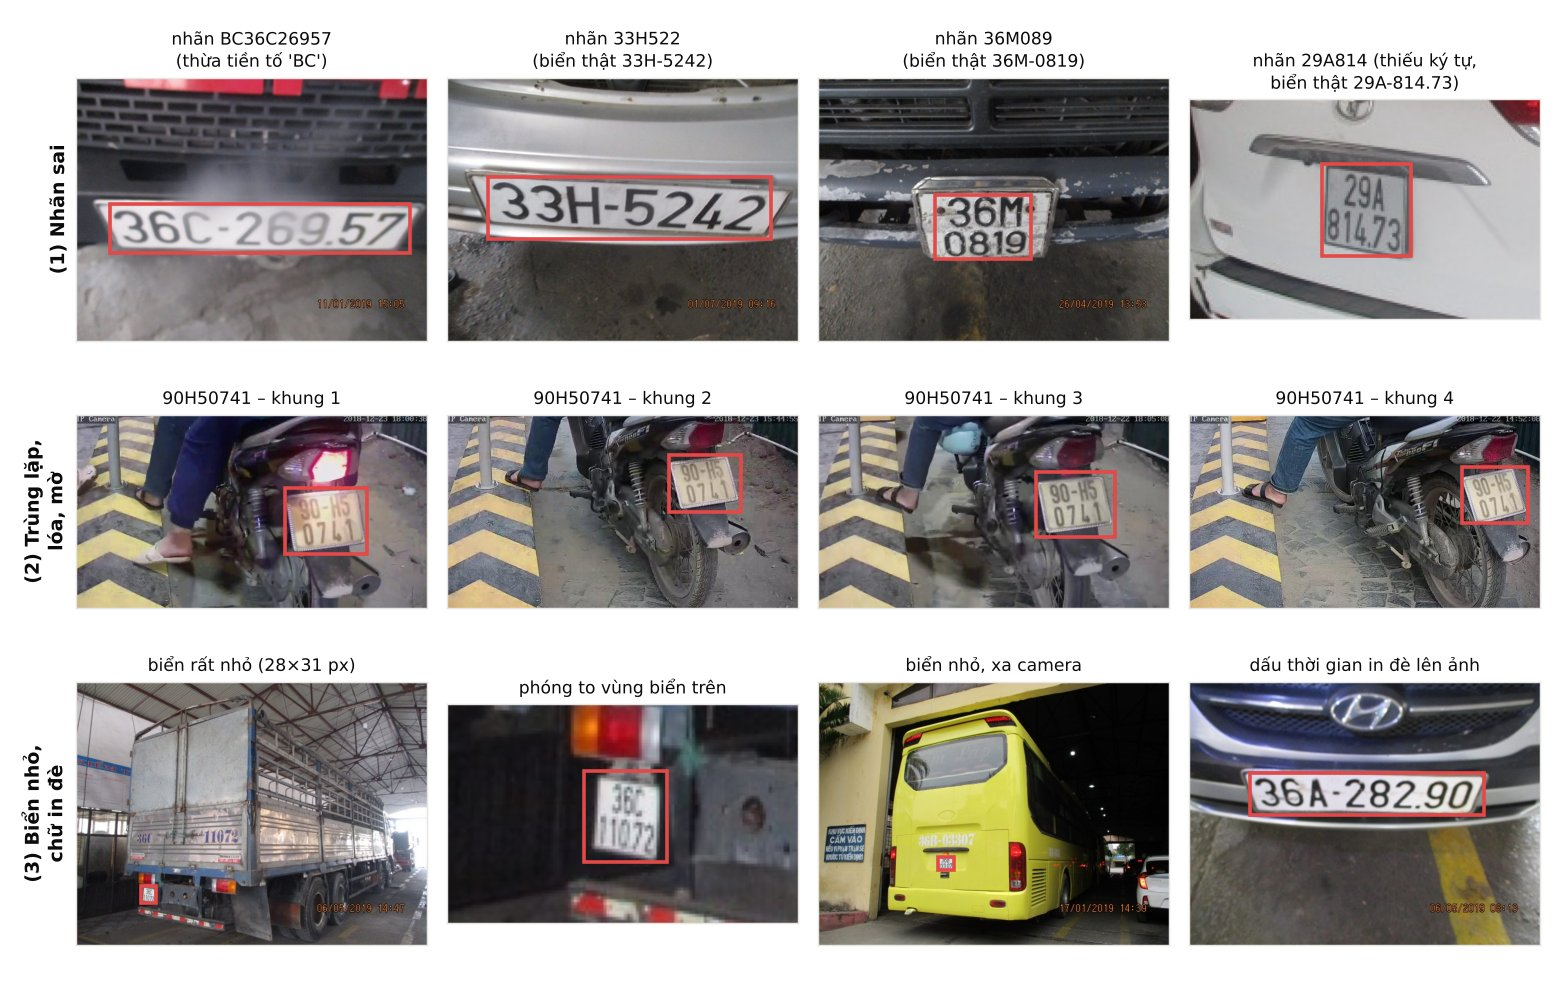
\includegraphics[width=\textwidth]{images/dataset/vnlp_issues.jpg}
\caption{Một số vấn đề của tập VNLP: nhãn sai, khung hình trùng lặp và lóa sáng, biển rất nhỏ, chữ in đè lên ảnh}
\label{fig:vnlp_issues}
\end{figure}

\begin{table}[H]
\centering
\small
\begin{tabularx}{\textwidth}{|>{\RaggedRight}p{3.3cm}|>{\RaggedRight}X|>{\RaggedRight\arraybackslash}p{5.0cm}|}
\hline
\textbf{Vấn đề} & \textbf{Biểu hiện, số liệu} & \textbf{Ảnh hưởng} \\
\hline
1. Lệch miền dữ liệu (domain gap) & Ảnh chụp trong nhà đăng kiểm, xe đứng yên, ánh sáng ổn định; không có cảnh đường phố, ban đêm, mưa; không có video ô tô & Mô hình đạt điểm cao trên VNLP nhưng có thể giảm mạnh khi chạy trên camera giao thông thật \\
\hline
2. Mất cân bằng mã tỉnh & 74,2\% biển mã 36 & Mô hình OCR thiên vị ký tự ``3'', ``6'' ở hai vị trí đầu, đọc kém biển tỉnh khác \\
\hline
3. Trùng lặp biển số & 29.304 ảnh (78,6\%) có biển số trùng với ít nhất một ảnh khác: cùng một ô tô chụp cả đầu và đuôi xe ở hai thư mục (10.465 biển); xe máy có biển xuất hiện tới 9 lần (khung hình liên tiếp) & Nếu chia ngẫu nhiên từng ảnh theo tỷ lệ 80/10/10, khoảng 66\% ảnh kiểm thử có cùng biển số trong tập huấn luyện; kết quả bị thổi phồng \\
\hline
4. Nhãn sai & 59 nhãn không khớp định dạng biển Việt Nam; đối chiếu từng ảnh: 37 nhãn sai (thừa chữ số như \texttt{36A041270}, thừa tiền tố như \texttt{BC36C26957}, thiếu ký tự như \texttt{29A814}, \texttt{33H522}), 21 nhãn đúng nhưng là định dạng đặc biệt, 1 nhãn không đọc được & Gây nhiễu khi huấn luyện OCR, làm sai lệch độ đo \\
\hline
5. Nhãn không đồng nhất & 3.715 nhãn dùng chữ thường (\texttt{29g141081}), chủ yếu ở nhóm xe máy & Nếu không chuẩn hóa, mô hình phải học hai lớp cho cùng một chữ cái \\
\hline
6. Tài liệu ghi sai định dạng tọa độ & Ghi $(x, y, w, h)$ nhưng thực tế là $(x_{\min}, y_{\min}, x_{\max}, y_{\max})$ & Chuyển đổi sai sẽ làm hỏng toàn bộ nhãn detection \\
\hline
7. Biển rất nhỏ, ảnh nhiễu & Biển 2 dòng ô tô chỉ chiếm khoảng 9\% chiều rộng ảnh; ảnh xe máy bị lóa đèn hậu, mờ; dấu thời gian in đè trên ảnh & Thách thức cho detector và OCR, nhưng cũng là dữ liệu khó có ích cho huấn luyện \\
\hline
\end{tabularx}
\caption{Tổng hợp các vấn đề của tập dữ liệu VNLP}
\label{tab:vnlp_issues}
\end{table}

\subsection{Hướng xử lý dữ liệu}

Từ các vấn đề trên, nhóm đề ra quy trình xử lý dữ liệu như Bảng~\ref{tab:vnlp_solutions}.

\begin{table}[H]
\centering
\small
\begin{tabularx}{\textwidth}{|>{\centering}p{0.8cm}|>{\RaggedRight\arraybackslash}X|}
\hline
\textbf{Vấn đề} & \textbf{Hướng xử lý} \\
\hline
1 & Xây dựng thêm 300--1.000 khung hình từ nguồn bên ngoài VNLP: video giao thông Việt Nam công khai có giấy phép phù hợp (ví dụ Creative Commons) và các bộ dữ liệu công khai khác (Roboflow Universe, GreenParking), ưu tiên cảnh đường phố, ban đêm, trời mưa; gán nhãn bằng Roboflow hoặc CVAT và loại các ảnh trùng với VNLP. Bộ này dùng làm \textbf{tập kiểm thử thực tế} độc lập; một phần nhỏ có thể dùng tinh chỉnh detector. Kết quả được báo cáo riêng trên tập VNLP và trên tập thực tế. \\
\hline
2 & Báo cáo độ chính xác riêng cho nhóm biển mã 36 và nhóm mã tỉnh khác. Khi huấn luyện OCR, cân nhắc lấy mẫu lại (oversampling) các biển ngoài mã 36 và tạo thêm ảnh biển tổng hợp với mã tỉnh ngẫu nhiên. \\
\hline
3 & \textbf{Chia train/val/test theo chuỗi biển số} (group split): mọi ảnh của cùng một biển (kể cả ảnh đầu xe và đuôi xe của cùng một ô tô) chỉ nằm trong một tập. Tỷ lệ 80/10/10, phân tầng theo ba nhóm dữ liệu. \\
\hline
4 & Kiểm tra mọi nhãn bằng biểu thức chính quy theo định dạng biển (ô tô, xe máy, xe máy điện, xe máy kiểu cũ, biển nước ngoài); đối chiếu từng nhãn không khớp với ảnh. Đã sửa 37 nhãn sai (Hình~\ref{fig:vnlp_label_fixes}); nhãn không đọc được bị loại khỏi tập OCR nhưng vẫn giữ cho detection. Kiểm tra thêm 89 ảnh mẫu có nhãn đúng định dạng: không phát hiện nhãn sai. \\
\hline
5 & Chuẩn hóa toàn bộ nhãn về chữ in hoa, bộ ký tự gồm 10 chữ số và các chữ cái dùng trên biển Việt Nam. \\
\hline
6 & Viết script chuyển đổi đọc tọa độ theo định dạng hai góc, vẽ ngẫu nhiên 50 ảnh để kiểm tra trực quan trước khi huấn luyện. \\
\hline
7 & Giữ lại ảnh khó; huấn luyện detector ở kích thước 640 để không mất biển nhỏ. Tăng cường dữ liệu trực tuyến trong lúc huấn luyện (mờ chuyển động, đổi sáng, nhiễu, xoay nhẹ) thay vì tạo sẵn ảnh tăng cường. \\
\hline
\end{tabularx}
\caption{Hướng xử lý tương ứng với từng vấn đề dữ liệu}
\label{tab:vnlp_solutions}
\end{table}

\begin{figure}[H]
\centering
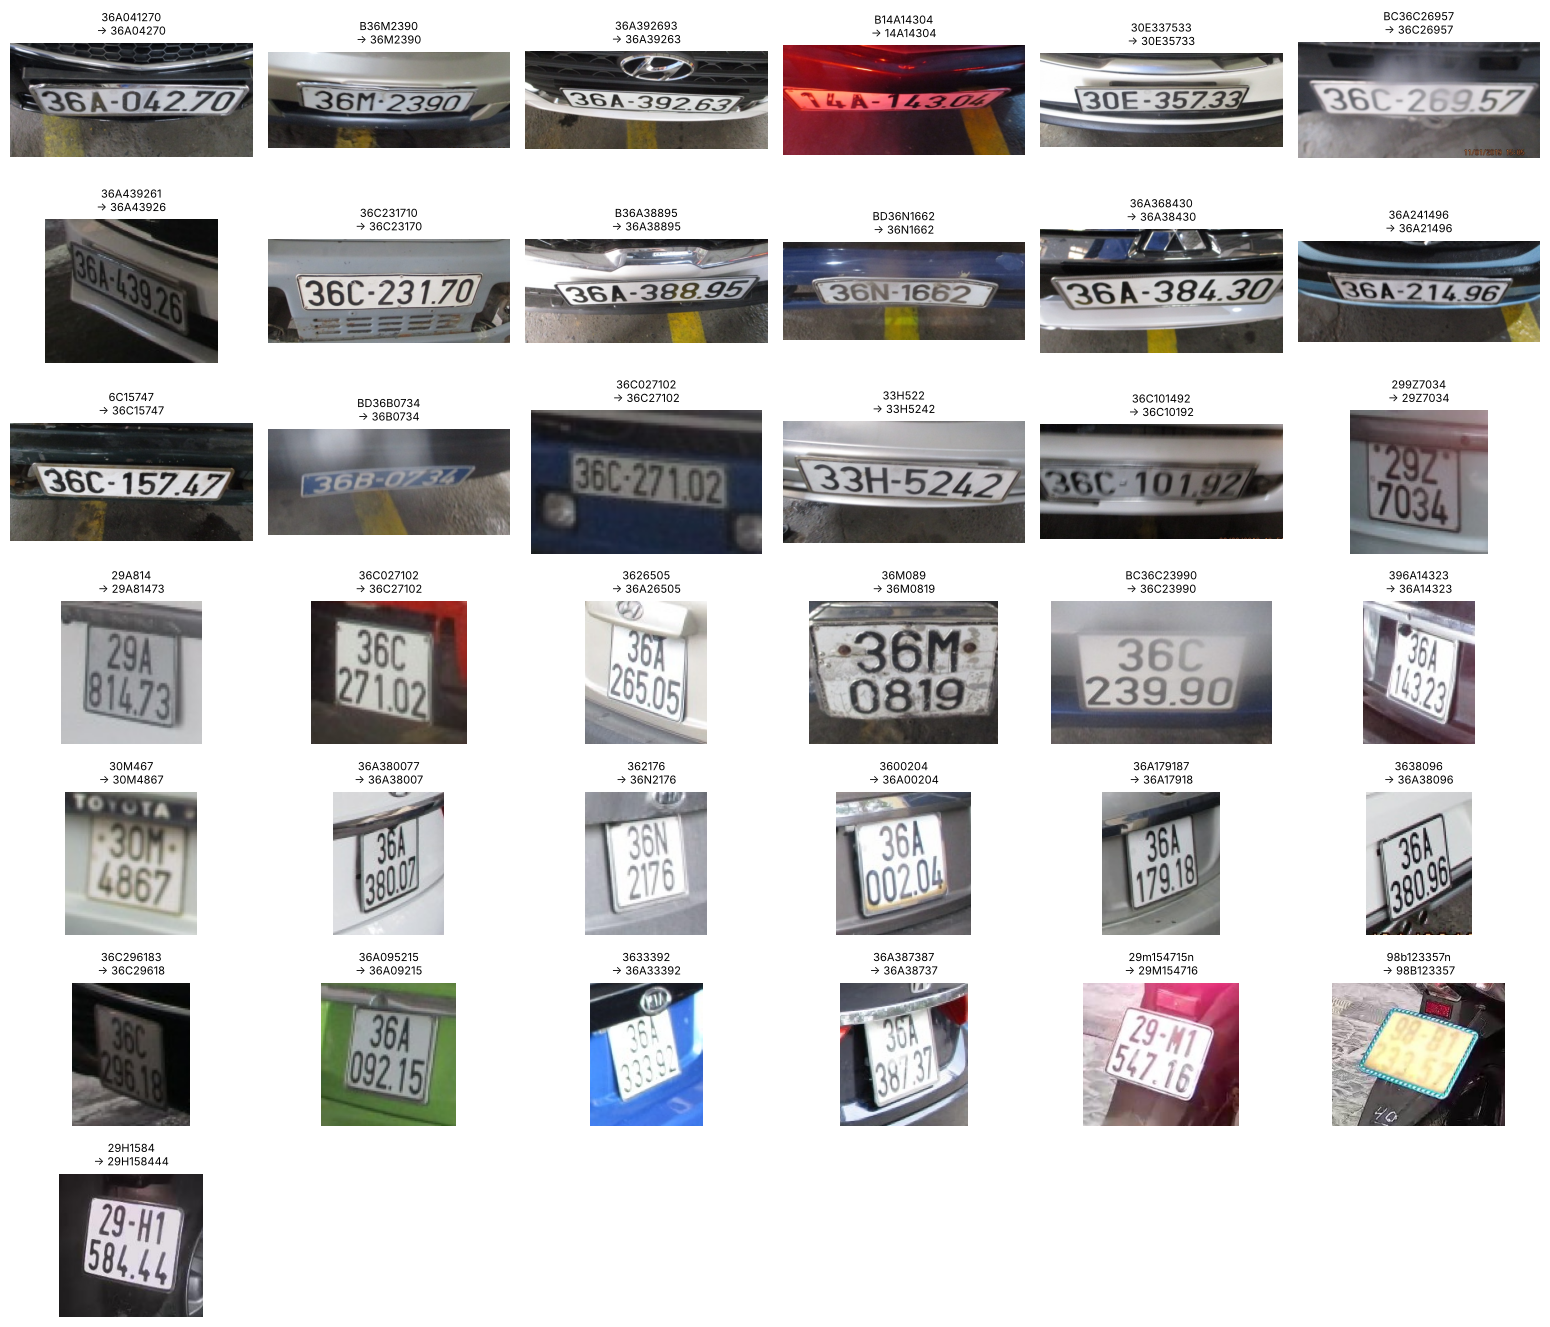
\includegraphics[width=0.95\textwidth]{images/dataset/vnlp_label_fixes.png}
\caption{37 nhãn sai đã được sửa: dòng trên là nhãn gốc, dòng dưới là nhãn sau khi đối chiếu với ảnh}
\label{fig:vnlp_label_fixes}
\end{figure}

Sau xử lý, từ VNLP sinh ra hai bộ dữ liệu dùng chung một cách chia:
\begin{enumerate}
  \item \textbf{Bộ detection:} ảnh gốc kèm tệp nhãn YOLO \texttt{(class, x\_center, y\_center, w, h)} chuẩn hóa về $[0, 1]$, gồm 2 lớp: \texttt{plate\_1row} và \texttt{plate\_2row}.
  \item \textbf{Bộ nhận dạng ký tự:} ảnh biển số được cắt theo hộp nhãn (thêm lề 3--5\%) kèm chuỗi ký tự đã chuẩn hóa.
\end{enumerate}

\section{Xác định đầu vào, đầu ra và yêu cầu của hệ thống}

\subsection{Đầu vào}

Hệ thống hỗ trợ ba loại đầu vào: ảnh tĩnh tải lên từ máy tính, tệp video và luồng webcam trực tiếp. Hệ thống cần hỗ trợ định dạng phổ biến (JPG, PNG, MP4) và thông báo rõ ràng khi tệp không hợp lệ hoặc không thể xử lý.

\subsection{Đầu ra}

Đầu ra dự kiến gồm:

\begin{itemize}
  \item Ảnh hoặc khung hình có vùng biển số được khoanh, kèm chuỗi ký tự hiển thị phía trên.
  \item Chuỗi biển số đã chuẩn hóa theo định dạng Việt Nam (ví dụ ``30A-123.45'').
  \item Điểm tin cậy của bước phát hiện và độ tin cậy của chuỗi ký tự.
  \item Với video: danh sách phương tiện kèm mã theo dõi, thời điểm xuất hiện và biển số cuối cùng sau tổng hợp.
  \item Thông báo phù hợp nếu không phát hiện được biển số hoặc không đọc được ký tự.
\end{itemize}

Cần phân biệt điểm tin cậy của mô hình phát hiện với xác suất chuỗi biển số được nhận dạng chính xác. Hai đại lượng này không đồng nghĩa với nhau.

\subsection{Yêu cầu chức năng}

Hệ thống cần đáp ứng các yêu cầu chức năng cơ bản:

\begin{enumerate}
  \item Cho phép tải ảnh, tải video hoặc mở webcam.
  \item Kiểm tra tính hợp lệ của tệp đầu vào.
  \item Phát hiện vị trí và loại biển số.
  \item Nhận dạng ký tự trên biển và chuẩn hóa theo định dạng biển Việt Nam.
  \item Theo dõi phương tiện và tổng hợp kết quả qua nhiều khung hình với đầu vào video.
  \item Hiển thị kết quả và lưu lịch sử nhận dạng.
  \item Cung cấp liên kết đến trang tra cứu vi phạm chính thức kèm biển số đã nhận dạng để người dùng tự tra cứu.
\end{enumerate}

\subsection{Yêu cầu phi chức năng}

\begin{itemize}
  \item \textbf{Độ chính xác:} hạn chế phát hiện nhầm và đọc sai ký tự; được đo trên cả tập VNLP và tập thực tế.
  \item \textbf{Thời gian thực:} xử lý webcam ở tốc độ từ 15 khung hình/giây trở lên trên máy tính xách tay của nhóm (mục tiêu sẽ được xác nhận bằng thực nghiệm).
  \item \textbf{Khả năng sử dụng:} giao diện web đơn giản, chạy được trên trình duyệt.
  \item \textbf{Chi phí triển khai:} sử dụng hạ tầng miễn phí, phù hợp với điều kiện sinh viên.
  \item \textbf{Bảo vệ dữ liệu:} biển số là dữ liệu liên quan đến cá nhân; hệ thống không chia sẻ ảnh, không tự động truy vấn hệ thống bên thứ ba.
\end{itemize}

\section{Lựa chọn công nghệ và giải pháp}

\subsection{Ngôn ngữ lập trình Python}

Python được lựa chọn làm ngôn ngữ chính do có hệ sinh thái phong phú cho thị giác máy tính và học sâu (PyTorch, OpenCV, Ultralytics), cho phép thực hiện toàn bộ quy trình từ xử lý dữ liệu, huấn luyện đến xây dựng dịch vụ trong một ngôn ngữ.

\subsection{OpenCV -- Xử lý ảnh}

OpenCV đảm nhiệm đọc ảnh và video, thay đổi kích thước, cắt vùng biển số và vẽ kết quả. OpenCV không tự giải quyết bài toán nhận dạng mà được kết hợp với các mô hình học sâu.

\subsection{YOLO và RT-DETR -- Phát hiện biển số}

Thư viện Ultralytics cung cấp cùng một giao diện huấn luyện cho các họ mô hình YOLO (YOLO11, YOLO26) và RT-DETR. Do mô hình huấn luyện sẵn trên tập COCO không có lớp biển số, nhóm tinh chỉnh các mô hình này trên tập VNLP đã chuyển đổi.

\subsection{Mô hình nhận dạng ký tự}

Các công cụ OCR tổng quát như Tesseract hay EasyOCR được thiết kế cho văn bản thông thường, thường đọc kém biển số 2 dòng. Nhóm dùng chúng làm mốc so sánh (baseline) và lựa chọn hướng chính là \textbf{huấn luyện mô hình nhận dạng cả biển} trên ảnh biển cắt từ VNLP (CRNN với hàm mất mát CTC, hoặc tinh chỉnh mô hình nhẹ chuyên cho biển số như \texttt{fast-plate-ocr}). Mô hình đọc cả biển trong một lần, không cần tách từng ký tự hay tách dòng.

\subsection{Giao diện và triển khai}

Giao diện được xây dựng dưới dạng ứng dụng web gồm máy chủ FastAPI xử lý ảnh, video và giao diện trình duyệt hiển thị kết quả. Mô hình được xuất sang định dạng ONNX để suy luận nhanh trên CPU hoặc GPU của máy cá nhân. Streamlit có thể dùng cho bản trình diễn nhanh trong giai đoạn đầu.

\subsection{Giải pháp tổng thể}

Giải pháp được lựa chọn là quy trình nhiều bước:

\begin{enumerate}
  \item \textbf{Tiếp nhận đầu vào:} ảnh, video hoặc khung hình webcam.
  \item \textbf{Phát hiện biển số:} mô hình phát hiện trả về hộp biển và loại biển.
  \item \textbf{Cắt và chuẩn hóa:} cắt vùng biển có thêm lề, đổi kích thước theo loại biển.
  \item \textbf{Nhận dạng ký tự:} mô hình nhận dạng trả về chuỗi và độ tin cậy.
  \item \textbf{Hậu xử lý:} kiểm tra và sửa theo định dạng biển Việt Nam.
  \item \textbf{Theo dõi và tổng hợp (với video):} gán mã cho từng xe, bỏ phiếu kết quả qua nhiều khung hình.
  \item \textbf{Hiển thị và lưu kết quả.}
\end{enumerate}

Thiết kế này tách rõ các thành phần, giúp kiểm thử từng bước và xác định nguyên nhân khi kết quả cuối cùng sai: do phát hiện, do vùng cắt hay do nhận dạng ký tự.

\section{Tiêu chí đánh giá hiệu quả giải pháp}

Hệ thống được đánh giá cả về khả năng phát hiện biển số và khả năng đọc đúng nội dung biển số.

Precision đo tỷ lệ dự đoán đúng trong tổng số dự đoán:
\[
  \mathrm{Precision} = \frac{TP}{TP + FP}
\]
Recall đo tỷ lệ biển số thực tế được phát hiện:
\[
  \mathrm{Recall} = \frac{TP}{TP + FN}
\]
trong đó TP là số biển phát hiện đúng, FP là số phát hiện nhầm và FN là số biển bị bỏ sót.

mAP@0.5 và mAP@0.5:0.95 đánh giá chất lượng hộp giới hạn; mAP@0.5:0.95 đặc biệt quan trọng vì hộp lệch có thể cắt mất ký tự sát mép.

Tỷ lệ đọc đúng toàn biển (Exact Match Accuracy) đo tỷ lệ mẫu có chuỗi dự đoán trùng hoàn toàn với nhãn:
\[
  \mathrm{Exact\ Match\ Accuracy} = \frac{\text{Số chuỗi đúng hoàn toàn}}{\text{Tổng số mẫu kiểm thử}}
\]

Ngoài ra, nhóm đo tỷ lệ lỗi ký tự (CER) và tốc độ xử lý (khung hình/giây). Mọi chỉ số được tính trên tập kiểm thử độc lập và \textbf{báo cáo riêng cho tập VNLP và tập thực tế}. Báo cáo chỉ trình bày kết quả thực nghiệm thực tế, không tự đặt ra giá trị khi chưa đánh giá.
